\section{Related work}
In this section we will discuss alternatives 

\subsection{Cassandra}
Cassandra scalable NoSQL database now available as open source through the Apache foundation. It was built from scratch with goal of being a massively scalable NoSQL database. In a cluster running Cassandra there is no sense of a master node, and all communication between nodes use peer to peer and the gossip protocol. As an administrator it is easy to scale Cassandra to meet both current and future system requirements. 

\subsubsection{Reads and writes}
In Cassandra all participating nodes can be accessed for writes and reads. To ensure durability all writes are preceded by a write to a commit log. If a node has crashed, a node holding a replica will service reads and writes according to the hinted handoff strategy. As with Voldemort, Cassandra also features tunable consistency. 

\subsubsection{Data model}
The Cassandra data model is based on a key:value model. However Cassandra extends this model with two levels of nesting. A database consists of column families. These families are comparable to how tables are in a normal relational database. With one level of nesting, which is mandatory, the datamodel will look something like this: key:[key:value, key:value ... key:value]. Now one put like this will act as one record in a normal database. If we take user data as a n example we could see something like this: primary_key:[name:smith, id:24, age:32].

\begin{figure}[h]
    \centering
    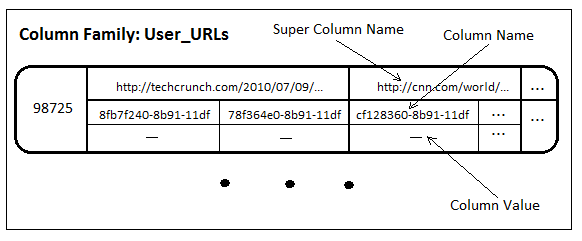
\includegraphics[width=0.5\textwidth]{resources/twitter-schema-user-urls.png}
    \caption{Hash ring with several nodes\cite{dynamo}.}
    \label{fig:hashring}
\end{figure}

As mentioned Cassandra also allows one more level of nesting. This 

column family: set of key-value pairs (a table with records)

key:value
value:list(key:value, key:value, key:value)


data model:
	-table family
	-super family
	-happy family

uses:
	facebook
	netflix
	spotify


\begin{figure}[ht]

\quad
\begin{minipage}[b]{0.45\linewidth}
    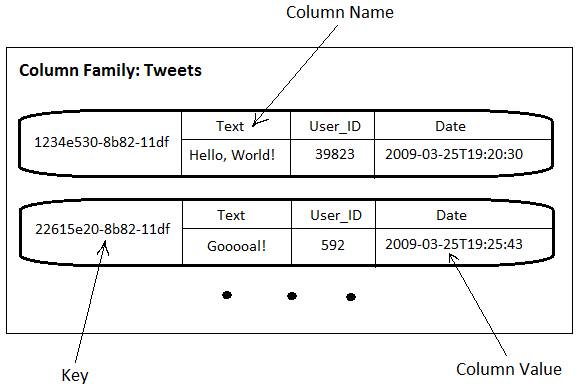
\includegraphics[width=1\textwidth]{resources/twitterschema-tweets.png}
    \caption{Front of the cluster}
    \label{fig:minipage2}
\end{minipage}
\end{figure}

what is it good for



limitations:
	
picture



\subsection{HBase}

\subsection{Bone dry servey that explains performance}
